% Supplementary detail preserved before main-text length balancing.
% This fragment is not included in the main manuscript.
\subsection{Component Isolation (Grounding Modality Ablation)}
\label{sec:exp2}

This ablation isolates which retrieved content is shown to the inference model: the raw episode, the accepted reflection, or both. The same retrieved tuples are used across conditions to reduce retrieval-quality confounding.

To achieve this, we evaluate the framework under three distinct ablation conditions. The first condition is \textit{Hybrid Grounding (VLEG)}, which represents the complete proposed methodology where the reasoning module is conditioned on both the retrieved raw episodes $e_i$ and their corresponding verified reflections $r_i^*$. The second condition is \textit{Abstract-Only Grounding}, where the reasoning module is provided solely with the verified reflections $r_i^*$, completely omitting the raw traffic episodic data. The third condition is \textit{Raw-Only Grounding}, which serves as a baseline mirroring standard In-Context Learning (ICL) \cite{brown2020language}, where the model receives only the raw episodes $e_i$ without any distilled semantic guidance.

To isolate the effect of grounding \emph{content} from retrieval quality, all three conditions retrieve the same top-$k$ memory tuples (via cosine similarity on the verified reflection's embedding, as VLEG's memory bank is built the same way regardless of which fields are shown at inference); only which fields of each retrieved tuple are shown to the reasoning LLM differs between conditions.

The measured results, shown in Figure \ref{fig:exp2_ablation}, do not match the hypothesized ordering. On Level 2 (no masking), Hybrid Grounding is indeed the best condition (87.5\% vs.\ 81.2\% for both alternatives). But on Level 3 --- the condition this experiment was specifically designed to stress-test --- the ordering inverts: Hybrid Grounding is the \emph{worst} of the three conditions, both overall (73.8\% pooled across 5 masking seeds, $n=80$, vs.\ 78.8\% for Abstract-Only and 75.0\% for Raw-Only) and specifically on the masked combinations that never appeared during memory formation (60.0\% pooled, $n=20$, vs.\ 70.0\% for both alternatives). Hybrid never outperformed both alternatives on Level 3 in any of the 5 seeds tested. We connect this to the memory-quality assessment (Section~\ref{sec:exp5}): verified reflections frequently cite causally irrelevant attributes as if they were determinative (see the empirical caveat in Section~\ref{sec:vleg-methodology}), and pairing a raw episode with such a reflection appears to anchor the reasoning model on the reflection's stated --- sometimes spurious --- condition rather than letting it reason more freely from the raw examples, which is more costly precisely when generalization to an unseen combination is required.

\begin{figure}[!t]
    \centering
    \begin{adjustbox}{max width=\linewidth}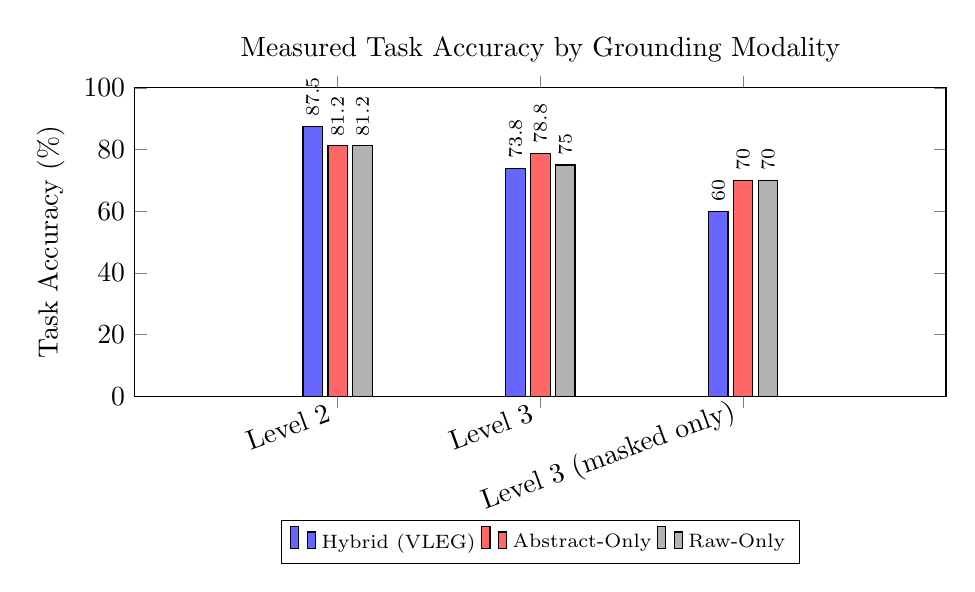
\begin{tikzpicture}
        \begin{axis}[
            ybar=2pt,
            bar width=7pt,
            width=0.98\linewidth,
            height=5.5cm,
            enlarge x limits=0.5,
            ylabel={Task Accuracy (\%)},
            ymin=0, ymax=100,
            symbolic x coords={Level 2, Level 3, Level 3 (masked only)},
            xtick=data,
            x tick label style={rotate=20, anchor=east},
            nodes near coords,
            nodes near coords align={vertical},
            every node near coord/.append style={font=\scriptsize,rotate=90,anchor=west},
            legend style={at={(0.5,-0.4)}, anchor=north, legend columns=-1, font=\scriptsize},
            title={Measured Task Accuracy by Grounding Modality}
        ]

        % Hybrid Grounding
        \addplot[fill=blue!60] coordinates {(Level 2, 87.5) (Level 3, 73.8) (Level 3 (masked only), 60.0)};
        \addlegendentry{Hybrid (VLEG)}

        % Abstract-Only Grounding
        \addplot[fill=red!60] coordinates {(Level 2, 81.2) (Level 3, 78.8) (Level 3 (masked only), 70.0)};
        \addlegendentry{Abstract-Only}

        % Raw-Only Grounding
        \addplot[fill=gray!60] coordinates {(Level 2, 81.2) (Level 3, 75.0) (Level 3 (masked only), 70.0)};
        \addlegendentry{Raw-Only}

        \end{axis}
    \end{tikzpicture}\end{adjustbox}
    \caption{Measured Task Accuracy across grounding modalities (reduced-order reimplementation, Qwen2.5-7B-Instruct). Level 3 figures are pooled across 5 masking seeds ($n=80$ overall, $n=20$ for the masked-only subset). Hybrid Grounding wins on Level 2 but is the worst condition on Level 3, especially on the masked combinations it was intended to help with --- the opposite of the original hypothesis.}
    \label{fig:exp2_ablation}
\end{figure}

At 7B, abstract-only context exceeds hybrid context by $5.0$ percentage points overall and $10.0$ points on the masked subset. The result does not support a claim that hybrid context is necessary for this task. The reported 70B check below has a different overall ordering.

We repeated this experiment with Llama-3.3-70B-Instruct across the same 5 masking seeds. Unlike the memory-strategy, refinement and memory-quality comparisons, where the 7B result either reversed cleanly (memory-strategy and refinement comparisons) or stayed exactly as limited (the memory-quality assessment), this one produced a genuinely mixed picture. Pooled over 5 seeds ($n=80$ overall, $n=20$ masked-only): overall accuracy, Hybrid ($95.0\%$) now ties Raw-Only ($95.0\%$) for best, with Abstract-Only worst ($91.25\%$) --- the opposite of Abstract-Only's 7B standing. But on the masked-combo subset specifically, Abstract-Only remains the best modality ($85.0\%$ vs.\ $80.0\%$ for both alternatives) --- the same direction as the 7B finding, just with a narrower margin ($5$ points versus $10$). Per-seed masked accuracy for Abstract-Only was noisy ($100\%, 75\%, 50\%, 100\%, 100\%$ across the 5 seeds), with one seed accounting for most of its overall shortfall. We do not read this as either a clean confirmation or a clean reversal of the 7B finding: the specific claim that Hybrid is the worst modality overall does not hold at 70B, but the narrower claim that Abstract-Only retrieval has some edge specifically on unseen, masked combinations persists in direction across both scales, just less dramatically.


\subsection{Iterative Refinement Ablation}
\label{sec:exp3}

The refinement ablation tests whether increasing the refinement budget recovers rejected episodes and changes prediction accuracy. It does not assume that iteration or verification is necessary in every task.

Both $K=1$ and $K=3$ run the same generate-and-verify procedure. At $K=1$, the one rejected proposal leads to discarding the episode; at $K=3$, the generator can revise after critique. This is a refinement-budget ablation, not a verified-versus-unverified comparison. Both use the same model and hybrid inference.

Across five masking seeds, $K=3$ achieves $75.0\%$ overall accuracy ($60/80$) versus $63.75\%$ ($51/80$) for $K=1$, a difference of $11.25$ percentage points. Masked-only accuracy is $60.0\%$ ($12/20$) versus $50.0\%$ ($10/20$). The masked-only difference is zero in three seeds and positive in two. These counts are repeated evaluations under different memory masks, not eighty independent scenes.

The mechanism behind the gain is memory bank \emph{coverage}, not reasoning quality per reflection: across the 5 seeds, $K=1$'s memory bank retained only $42$--$58\%$ of training episodes (an episode whose first-guess reflection is rejected is discarded outright, since $j$ is never $<K{=}1$ again), while $K=3$'s retained $83$--$100\%$, because the critique from a rejected first attempt typically reveals the correct label and lets the generator correct itself on the second or third try. Verification at $K=3$ is thus better understood here as \emph{recovering episodes that a single unlucky guess would otherwise lose}, not as improving the causal quality of the reflections that do get committed --- see the memory-quality assessment (Section~\ref{sec:exp5}) for a direct measurement showing no such quality improvement.

At 70B, the reported mean overall difference is $26.2$ percentage points (standard deviation $8.1$) across the same five seeds, and $K=3$ admits all twelve historical episodes in each seed. The results are consistent with coverage recovery through label-informed critique; they do not show that the accepted explanations identify causal attributes more reliably.


\subsection{Parameter Sensitivity and Overhead Analysis}
\label{sec:exp4}

The primary objective of the parameter-sensitivity study is to systematically analyze the convergence behavior of the VLEG verification loop and to quantify the associated computational trade-offs. While the iterative generate-and-verify mechanism is designed to strictly filter out hallucinated heuristics, each refinement cycle inherently incurs additional computational costs during the memory consolidation phase. Therefore, it is critical to evaluate how the strictness of the verification process impacts both the downstream reasoning performance and the overall token efficiency of the system.

To conduct this sensitivity analysis, we manipulate the maximum refinement iterations parameter, $K$, across a discrete set of values: $K \in \{1, 2, 3, 5\}$. The condition $K=1$ effectively disables the iterative refinement loop, reducing the system to a single-step reflection generator akin to standard localized reflection baselines \cite{shinn2023reflexion}. For each configuration of $K$, we evaluate the model on both Level 2 and Level 3 of the Experience-Transfer task. We record the resulting Task Accuracy (\%) alongside the Computational Overhead, which is measured as the total number of prompt and completion tokens consumed per consolidated episodic memory.

\begin{figure*}[!t]
    \centering
    \begin{adjustbox}{max width=\linewidth}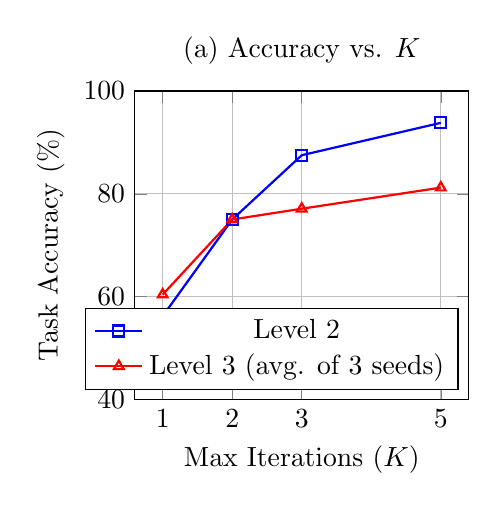
\begin{tikzpicture}
        \begin{axis}[
            width=0.48\linewidth,
            height=5.5cm,
            xlabel={Max Iterations ($K$)},
            ylabel={Task Accuracy (\%)},
            ymin=40, ymax=100,
            xtick={1,2,3,5},
            grid=major,
            legend pos=south east,
            title={(a) Accuracy vs. $K$}
        ]
        \addplot[color=blue, mark=square, thick] coordinates {(1, 56.2) (2, 75.0) (3, 87.5) (5, 93.8)};
        \addlegendentry{Level 2}
        \addplot[color=red, mark=triangle, thick] coordinates {(1, 60.4) (2, 75.0) (3, 77.1) (5, 81.2)};
        \addlegendentry{Level 3 (avg. of 3 seeds)}
        \end{axis}
    \end{tikzpicture}\end{adjustbox}
    \hfill
    \begin{adjustbox}{max width=\linewidth}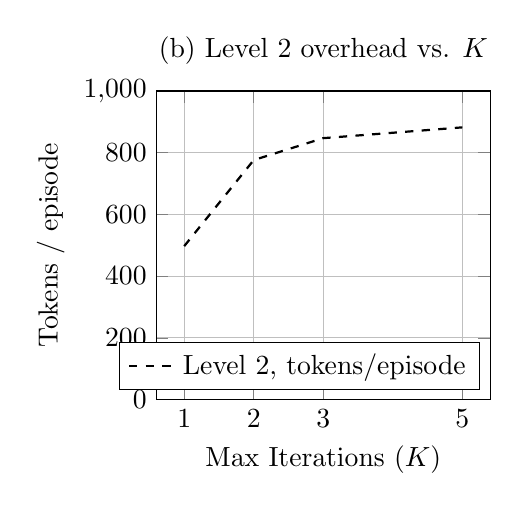
\begin{tikzpicture}
        \begin{axis}[
            width=0.48\linewidth,
            height=5.5cm,
            xlabel={Max Iterations ($K$)},
            ylabel={Tokens / episode},
            ymin=0, ymax=1000,
            xtick={1,2,3,5},
            grid=major,
            legend pos=south east,
            title={(b) Level 2 overhead vs. $K$}
        ]
        \addplot[color=black, mark=circle, thick, dashed] coordinates {(1, 497) (2, 776) (3, 847) (5, 882)};
        \addlegendentry{Level 2, tokens/episode}
        \end{axis}
    \end{tikzpicture}\end{adjustbox}
    \caption{Measured parameter sensitivity of the maximum refinement iterations $K$ (reduced-order reimplementation, Qwen2.5-7B-Instruct). (a) Task Accuracy does \emph{not} plateau at $K=3$: Level 2 (a single deterministic run, confirmed identical on repeat) keeps improving through $K=5$; Level 3 (averaged over 3 masking seeds) plateaus in only 1 of 3 seeds individually. (b) Token overhead per consolidated episode is concave, not linear: most of the cost increase happens between $K{=}1$ and $K{=}2$, with sharply diminishing marginal cost for extending the budget further, since only a minority of episodes ever use the additional iterations.}
    \label{fig:exp4_sensitivity}
\end{figure*}

The measured results, shown in Figure \ref{fig:exp4_sensitivity}, contradict both claims originally hypothesized for this experiment. First, Task Accuracy does not plateau around $K=3$. On Level 2 --- a single run, verified deterministic by an exact repeat --- accuracy keeps climbing substantially from $K{=}3$ ($87.5\%$) to $K{=}5$ ($93.8\%$), a further $+6.3$ point gain with no sign of leveling off in this range. On Level 3, we tested 3 independent masking seeds: only one of them ($\text{seed}=42$) shows the exact plateau signature (identical bank composition, token count, and accuracy at $K{=}3$ and $K{=}5$); the other two show $K{=}5$ either matching or beating $K{=}3$ by a further $+6$--$12.5$ points. We do not have a reliable stopping criterion at $K=3$ in this environment --- it happens to be sufficient for some random draws of the masked subset and insufficient for others.

Second, Computational Overhead does not scale linearly with $K$. It is concave: the token cost per consolidated episode rises sharply from $K{=}1$ to $K{=}2$ ($+279$ tokens/episode on Level 2) and then far more slowly for each additional unit of $K$ budget ($+71$ tokens/episode from $K{=}2$ to $K{=}3$, $+35$ from $K{=}3$ to $K{=}5$ despite that step covering two extra iterations, not one). This pattern was consistent across all seeds tested on both levels. The mechanism is straightforward: most episodes converge within 1--2 iterations regardless of the ceiling $K$; raising the ceiling only adds cost for the small minority of episodes that are still unresolved at iteration 3, so the marginal cost of a higher $K$ budget shrinks as $K$ grows even as the marginal \emph{benefit} (per the accuracy panel) does not reliably shrink in the same way. Practitioners should not treat $K=3$ as a validated efficiency-optimal cutoff on the basis of this experiment; whether a higher $K$ is worth its (modest, sub-linear) additional cost depends on how much the specific downstream task benefits from the extra recovered episodes, which the refinement ablation (Section~\ref{sec:exp3}) suggests is real but seed-dependent in magnitude.

At 70B, the reported Level-3 sweep uses three masking seeds. In each, $K=2$, $K=3$ and $K=5$ yield the same admitted memory, token consumption and accuracy. No episode needs a third attempt in these runs. The observed plateau is therefore at $K=2$ in this model and task, while the 7B sweep is less uniform. This does not establish a universal stopping budget.

Concurrent GPU workloads make the affected timing measurements unsuitable for a clean overhead comparison. One reported repeat at Level 2, $K=3$, changes the token count from $12{,}541$ to $12{,}625$ while preserving accuracy. Accordingly, temperature $0$ is recorded as a decoding setting, and repeatability and hardware contention must be assessed empirically for each run.


\subsection{Public-Flow Benchmark Validation}
\label{sec:exp6}
This experiment tests whether local verification and hybrid memory improve classification of independent public flow records. It uses UNSW-NB15, a captured testbed benchmark containing normal and generated attack traffic \cite{moustafa2015unsw}. It is not a production deployment or zero-day detection study. The completed archive contains 500 pilot predictions and 25,000 formal predictions; an offline audit reproduces the metrics, conditional bootstrap intervals and construction-cost totals from the stored records.

The source partitions contain 175,341 historical and 82,332 test records. The frozen feature representation uses nineteen fields: duration, protocol, service, state, directional packet and byte counts, rate, TTL, load, inter-packet timing, jitter and mean packet size. IPs, timestamps, row identifiers, attack names and target labels are excluded from model inputs and retrieval keys. The public mirror is pinned to a commit; its file names are reversed relative to the official partition sizes, so role mapping is recorded explicitly and checked by row count, size, MD5 and SHA256. Bytes agree with an independent research deposit, although the original author-hosted files were not directly accessible.

Identical selected-feature vectors sometimes have conflicting labels. We exclude every row in such groups rather than choosing a label: 6,896 historical rows in 273 groups and 2,912 test rows in 105 groups. We also remove 79,746 and 33,161 remaining same-label duplicate rows, respectively, leaving 88,699 historical and 46,259 test fingerprints. A further 1,044 test fingerprints overlap the cleaned historical source and are excluded. Thus the evaluated population is deduplicated and unambiguous in this representation; removing these cases can change difficulty and class balance, so these results do not estimate performance on the original flow-frequency distribution. Session-level independence cannot be established because this partition lacks session-group metadata.

Each of five memory seeds (20261020--20261024) selects sixteen benign and sixteen malicious historical examples. They share the same 1,000 test fingerprints: 663 benign and 337 malicious. The 100 pilot queries do not overlap these formal queries. We use Llama-3.3-70B (70.6B parameters, Q4\_K\_M), nomic-embed-text (137M, F16), temperature $0$, $K=3$, $k=3$, and a 32,768-token chat-context ceiling. The run records exact model digests, source/code hashes and Python 3.13.13; the server has two A800 80GB GPUs. Generator and verifier are separate calls to the same model. Historical labels are available to verification and the raw baseline, but target labels are used only after inference for scoring. The generator's first proposal receives only historical flow features.

The five conditions are raw flow retrieval, an unverified first reflection, VLEG, raw flow retrieval restricted to VLEG's admitted examples, and a single global summary of the labeled historical memory. All local conditions share a label-free raw-feature embedding retrieval pass and the same selected top-three candidates. A rejected candidate is dropped without replacement. The raw-on-admitted control therefore removes reflection content while retaining the same admission mask as VLEG. This shared raw retrieval deliberately differs from the reflection-driven formulation in Section III and tests consolidation/admission under controlled retrieval; it does not evaluate every component of the full formulation. Global-summary inference sees a corpus summary rather than the same top-three examples, and is a memory-architecture comparison rather than an equal-evidence modality ablation. These are controlled adaptations, not complete published Reflexion/HDR reproductions.

\begin{table*}[!t]
\centering
\caption{Public-flow performance, mean $\pm$ sample standard deviation across five historical-memory seeds (percent). All seeds use the same 1,000 test fingerprints. Invalid outputs count as errors.}
\label{tab:exp6_performance}
\small
\begin{tabular}{lrrrr}
\toprule
Condition & Accuracy & Macro-F1 & Attack recall & False positive rate \\
\midrule
Raw flow retrieval & 65.08 $\pm$ 2.93 & 63.92 $\pm$ 2.54 & 71.39 $\pm$ 8.44 & 38.13 $\pm$ 6.85 \\
Unverified single-step & 61.38 $\pm$ 1.08 & 42.66 $\pm$ 1.35 & 6.17 $\pm$ 1.43 & 9.89 $\pm$ 2.03 \\
VLEG & 59.74 $\pm$ 2.03 & 59.68 $\pm$ 2.03 & 77.74 $\pm$ 5.69 & 48.78 $\pm$ 1.67 \\
Raw on admitted flows & 64.86 $\pm$ 2.96 & 63.70 $\pm$ 2.68 & 71.16 $\pm$ 8.71 & 38.34 $\pm$ 6.61 \\
Global summary & 50.22 $\pm$ 12.45 & 47.60 $\pm$ 14.13 & 87.12 $\pm$ 22.27 & 68.54 $\pm$ 24.20 \\
\bottomrule
\end{tabular}
\end{table*}

Table~\ref{tab:exp6_performance} and Figure~\ref{fig:exp6_tradeoff} show that raw retrieval has the highest mean Macro-F1 among the evaluated conditions ($63.92\%$), while VLEG reaches $59.68\%$. VLEG increases attack recall from $71.39\%$ to $77.74\%$, but increases the false positive rate from $38.13\%$ to $48.78\%$. Its accuracy falls from $65.08\%$ to $59.74\%$. A post hoc always-benign reference has accuracy $66.30\%$, Macro-F1 $39.87\%$ and zero attack recall; this illustrates why accuracy alone is insufficient here. None of these conditions establishes deployment-quality intrusion detection, and no comparison against a trained conventional intrusion classifier is made.

Verification is beneficial relative to the unverified first-reflection condition: Macro-F1 improves by $17.02$ percentage points, and attack recall rises from $6.17\%$ to $77.74\%$. However, high admitted-memory coverage ($98.75\%$, 158/160 historical episodes) does not establish reliable cross-flow explanations. Raw-on-admitted retrieval nearly matches the raw baseline ($63.70\%$ versus $63.92\%$ Macro-F1), whereas adding the accepted reflections reduces its mean score to $59.68\%$. These comparisons are consistent with reflection content changing the decision trade-off; they do not establish a specific anchoring or causal-attribution mechanism. A subsequent deterministic explanation screen finds source-label agreement in 158/158 admitted VLEG reflections versus 84/160 first proposals. Explicit conjunctive conditions can be evaluated in 157/158 VLEG reflections; all 157 hold on their source flow, but 113 have at least one contrary-label match among the other archived historical draws. The remaining expression uses ambiguous $\gg$ syntax and is unresolved. The screen uses 160 unique historical flows and no test queries. It checks literal predicates, not natural-language causal validity, and the historical pool is neither independent nor representative. A human review with field-semantic judgments and adjudication remains incomplete.

\begin{figure*}[!t]
\centering
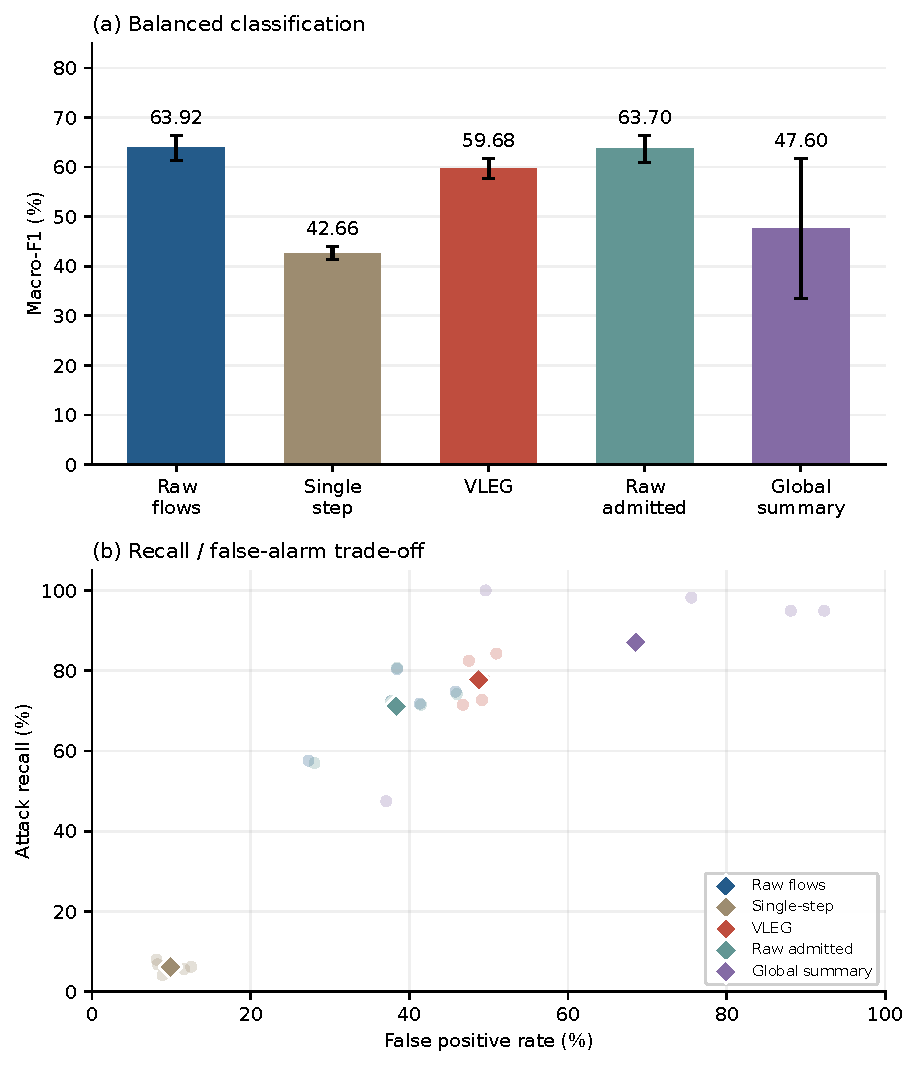
\includegraphics[width=0.94\textwidth]{exp6_tradeoff.pdf}
\caption{Public-flow results across five memory seeds. Left: mean Macro-F1 with sample-standard-deviation bars. Right: attack recall versus false positive rate; faint points are individual seeds and large markers are means. The larger recall of VLEG is accompanied by more false alarms.}
\label{fig:exp6_tradeoff}
\end{figure*}

A paired bootstrap resamples the same 1,000 fingerprints synchronously across methods and all five memory seeds (1,000 replicates). The mean VLEG-minus-raw Macro-F1 difference is $-4.24$ percentage points, with a conditional 95\% interval of $[-5.91,-2.53]$; VLEG is lower in four seeds and slightly higher in one. VLEG-minus-single-step is $+17.02$ points, interval $[13.71,20.39]$. VLEG-minus-raw-on-admitted is $-4.02$ points, interval $[-5.79,-2.28]$. These are unadjusted descriptive intervals conditional on the fixed memory draws and an assumption of independent fingerprints; they do not quantify uncertainty over new networks, sessions, model weights or memory-seed populations. Five repeated evaluations do not create 5,000 independent test flows. Per-attack recalls are archived, but rare categories include only one Backdoor, one Worms and three Shellcode cases; their percentages cannot support precise category-specific conclusions.

Table~\ref{tab:exp6_cost} separates one-time memory construction from query chat time. VLEG uses a mean 40,094 construction tokens and 419.43 seconds, versus 9,405 tokens and 126.54 seconds for first-proposal reflections. Raw storage needs no construction chat calls; embedding cost is separate and embedding tokens are not included. VLEG query input averages 909 tokens versus 780 for raw retrieval. Methods run in the fixed order raw, single-step, VLEG, raw-on-admitted, global summary. Consequently, prompt caching and order confound latency comparisons: the shorter observed VLEG chat time is not evidence of a causal speed advantage. Moreover, among 4,968 raw/raw-on-admitted pairs with identical reconstructed prompts, 24 predictions differ despite temperature $0$. This variation limits interpretation of the small raw-versus-admission-control gap. There are 29 invalid single-step outputs and 30 invalid VLEG outputs across 5,000 predictions each; all other conditions have zero invalid outputs. False positive rate counts explicit malicious predictions on benign flows, so invalid-output counts and benign recall must be considered alongside it.

\begin{table*}[!t]
\centering
\caption{Observed public-flow costs, means across five memory seeds. Construction tokens include input and output. Chat latency excludes shared retrieval and is confounded by fixed method order/cache reuse.}
\label{tab:exp6_cost}
\small
\begin{tabular}{lrrrrr}
\toprule
Condition & Construction calls & Construction tokens & Construction (s) & Query mean (s) & Query p95 (s) \\
\midrule
Raw flow retrieval & 0 & 0 & 0 & 2.12 & 2.67 \\
Unverified single-step & 32.0 & 9,405 & 126.54 & 2.23 & 2.75 \\
VLEG & 120.4 & 40,094 & 419.43 & 1.74 & 2.68 \\
Raw on admitted flows & 120.4 & 40,094 & 419.43 & 0.95 & 1.19 \\
Global summary & 1.0 & 5,947 & 23.21 & 1.21 & 1.30 \\
\bottomrule
\end{tabular}
\end{table*}
The admission-control condition shares VLEG's construction process and its cost; it does not obtain the mask for free. The completed experiment therefore supports a bounded result: checking first reflections improves on an unverified adaptation, but accepted hybrid reflections do not improve balanced classification over raw retrieval on this cleaned public-flow population.

